% Generated by Sphinx.
\def\sphinxdocclass{report}
\documentclass[letterpaper,10pt,english]{sphinxmanual}
\usepackage[utf8]{inputenc}
\DeclareUnicodeCharacter{00A0}{\nobreakspace}
\usepackage[T1]{fontenc}
\usepackage{babel}
\usepackage{times}
\usepackage[Bjarne]{fncychap}
\usepackage{longtable}
\usepackage{sphinx}


\title{mplot documentation}
\date{November 19, 2011}
\release{0.9.6}
\author{Matthew Newville}
\newcommand{\sphinxlogo}{}
\renewcommand{\releasename}{Release}
\makeindex

\makeatletter
\def\PYG@reset{\let\PYG@it=\relax \let\PYG@bf=\relax%
    \let\PYG@ul=\relax \let\PYG@tc=\relax%
    \let\PYG@bc=\relax \let\PYG@ff=\relax}
\def\PYG@tok#1{\csname PYG@tok@#1\endcsname}
\def\PYG@toks#1+{\ifx\relax#1\empty\else%
    \PYG@tok{#1}\expandafter\PYG@toks\fi}
\def\PYG@do#1{\PYG@bc{\PYG@tc{\PYG@ul{%
    \PYG@it{\PYG@bf{\PYG@ff{#1}}}}}}}
\def\PYG#1#2{\PYG@reset\PYG@toks#1+\relax+\PYG@do{#2}}

\def\PYG@tok@gd{\def\PYG@tc##1{\textcolor[rgb]{0.63,0.00,0.00}{##1}}}
\def\PYG@tok@gu{\let\PYG@bf=\textbf\def\PYG@tc##1{\textcolor[rgb]{0.50,0.00,0.50}{##1}}}
\def\PYG@tok@gt{\def\PYG@tc##1{\textcolor[rgb]{0.00,0.25,0.82}{##1}}}
\def\PYG@tok@gs{\let\PYG@bf=\textbf}
\def\PYG@tok@gr{\def\PYG@tc##1{\textcolor[rgb]{1.00,0.00,0.00}{##1}}}
\def\PYG@tok@cm{\let\PYG@it=\textit\def\PYG@tc##1{\textcolor[rgb]{0.25,0.50,0.56}{##1}}}
\def\PYG@tok@vg{\def\PYG@tc##1{\textcolor[rgb]{0.73,0.38,0.84}{##1}}}
\def\PYG@tok@m{\def\PYG@tc##1{\textcolor[rgb]{0.13,0.50,0.31}{##1}}}
\def\PYG@tok@mh{\def\PYG@tc##1{\textcolor[rgb]{0.13,0.50,0.31}{##1}}}
\def\PYG@tok@cs{\def\PYG@tc##1{\textcolor[rgb]{0.25,0.50,0.56}{##1}}\def\PYG@bc##1{\colorbox[rgb]{1.00,0.94,0.94}{##1}}}
\def\PYG@tok@ge{\let\PYG@it=\textit}
\def\PYG@tok@vc{\def\PYG@tc##1{\textcolor[rgb]{0.73,0.38,0.84}{##1}}}
\def\PYG@tok@il{\def\PYG@tc##1{\textcolor[rgb]{0.13,0.50,0.31}{##1}}}
\def\PYG@tok@go{\def\PYG@tc##1{\textcolor[rgb]{0.19,0.19,0.19}{##1}}}
\def\PYG@tok@cp{\def\PYG@tc##1{\textcolor[rgb]{0.00,0.44,0.13}{##1}}}
\def\PYG@tok@gi{\def\PYG@tc##1{\textcolor[rgb]{0.00,0.63,0.00}{##1}}}
\def\PYG@tok@gh{\let\PYG@bf=\textbf\def\PYG@tc##1{\textcolor[rgb]{0.00,0.00,0.50}{##1}}}
\def\PYG@tok@ni{\let\PYG@bf=\textbf\def\PYG@tc##1{\textcolor[rgb]{0.84,0.33,0.22}{##1}}}
\def\PYG@tok@nl{\let\PYG@bf=\textbf\def\PYG@tc##1{\textcolor[rgb]{0.00,0.13,0.44}{##1}}}
\def\PYG@tok@nn{\let\PYG@bf=\textbf\def\PYG@tc##1{\textcolor[rgb]{0.05,0.52,0.71}{##1}}}
\def\PYG@tok@no{\def\PYG@tc##1{\textcolor[rgb]{0.38,0.68,0.84}{##1}}}
\def\PYG@tok@na{\def\PYG@tc##1{\textcolor[rgb]{0.25,0.44,0.63}{##1}}}
\def\PYG@tok@nb{\def\PYG@tc##1{\textcolor[rgb]{0.00,0.44,0.13}{##1}}}
\def\PYG@tok@nc{\let\PYG@bf=\textbf\def\PYG@tc##1{\textcolor[rgb]{0.05,0.52,0.71}{##1}}}
\def\PYG@tok@nd{\let\PYG@bf=\textbf\def\PYG@tc##1{\textcolor[rgb]{0.33,0.33,0.33}{##1}}}
\def\PYG@tok@ne{\def\PYG@tc##1{\textcolor[rgb]{0.00,0.44,0.13}{##1}}}
\def\PYG@tok@nf{\def\PYG@tc##1{\textcolor[rgb]{0.02,0.16,0.49}{##1}}}
\def\PYG@tok@si{\let\PYG@it=\textit\def\PYG@tc##1{\textcolor[rgb]{0.44,0.63,0.82}{##1}}}
\def\PYG@tok@s2{\def\PYG@tc##1{\textcolor[rgb]{0.25,0.44,0.63}{##1}}}
\def\PYG@tok@vi{\def\PYG@tc##1{\textcolor[rgb]{0.73,0.38,0.84}{##1}}}
\def\PYG@tok@nt{\let\PYG@bf=\textbf\def\PYG@tc##1{\textcolor[rgb]{0.02,0.16,0.45}{##1}}}
\def\PYG@tok@nv{\def\PYG@tc##1{\textcolor[rgb]{0.73,0.38,0.84}{##1}}}
\def\PYG@tok@s1{\def\PYG@tc##1{\textcolor[rgb]{0.25,0.44,0.63}{##1}}}
\def\PYG@tok@gp{\let\PYG@bf=\textbf\def\PYG@tc##1{\textcolor[rgb]{0.78,0.36,0.04}{##1}}}
\def\PYG@tok@sh{\def\PYG@tc##1{\textcolor[rgb]{0.25,0.44,0.63}{##1}}}
\def\PYG@tok@ow{\let\PYG@bf=\textbf\def\PYG@tc##1{\textcolor[rgb]{0.00,0.44,0.13}{##1}}}
\def\PYG@tok@sx{\def\PYG@tc##1{\textcolor[rgb]{0.78,0.36,0.04}{##1}}}
\def\PYG@tok@bp{\def\PYG@tc##1{\textcolor[rgb]{0.00,0.44,0.13}{##1}}}
\def\PYG@tok@c1{\let\PYG@it=\textit\def\PYG@tc##1{\textcolor[rgb]{0.25,0.50,0.56}{##1}}}
\def\PYG@tok@kc{\let\PYG@bf=\textbf\def\PYG@tc##1{\textcolor[rgb]{0.00,0.44,0.13}{##1}}}
\def\PYG@tok@c{\let\PYG@it=\textit\def\PYG@tc##1{\textcolor[rgb]{0.25,0.50,0.56}{##1}}}
\def\PYG@tok@mf{\def\PYG@tc##1{\textcolor[rgb]{0.13,0.50,0.31}{##1}}}
\def\PYG@tok@err{\def\PYG@bc##1{\fcolorbox[rgb]{1.00,0.00,0.00}{1,1,1}{##1}}}
\def\PYG@tok@kd{\let\PYG@bf=\textbf\def\PYG@tc##1{\textcolor[rgb]{0.00,0.44,0.13}{##1}}}
\def\PYG@tok@ss{\def\PYG@tc##1{\textcolor[rgb]{0.32,0.47,0.09}{##1}}}
\def\PYG@tok@sr{\def\PYG@tc##1{\textcolor[rgb]{0.14,0.33,0.53}{##1}}}
\def\PYG@tok@mo{\def\PYG@tc##1{\textcolor[rgb]{0.13,0.50,0.31}{##1}}}
\def\PYG@tok@mi{\def\PYG@tc##1{\textcolor[rgb]{0.13,0.50,0.31}{##1}}}
\def\PYG@tok@kn{\let\PYG@bf=\textbf\def\PYG@tc##1{\textcolor[rgb]{0.00,0.44,0.13}{##1}}}
\def\PYG@tok@o{\def\PYG@tc##1{\textcolor[rgb]{0.40,0.40,0.40}{##1}}}
\def\PYG@tok@kr{\let\PYG@bf=\textbf\def\PYG@tc##1{\textcolor[rgb]{0.00,0.44,0.13}{##1}}}
\def\PYG@tok@s{\def\PYG@tc##1{\textcolor[rgb]{0.25,0.44,0.63}{##1}}}
\def\PYG@tok@kp{\def\PYG@tc##1{\textcolor[rgb]{0.00,0.44,0.13}{##1}}}
\def\PYG@tok@w{\def\PYG@tc##1{\textcolor[rgb]{0.73,0.73,0.73}{##1}}}
\def\PYG@tok@kt{\def\PYG@tc##1{\textcolor[rgb]{0.56,0.13,0.00}{##1}}}
\def\PYG@tok@sc{\def\PYG@tc##1{\textcolor[rgb]{0.25,0.44,0.63}{##1}}}
\def\PYG@tok@sb{\def\PYG@tc##1{\textcolor[rgb]{0.25,0.44,0.63}{##1}}}
\def\PYG@tok@k{\let\PYG@bf=\textbf\def\PYG@tc##1{\textcolor[rgb]{0.00,0.44,0.13}{##1}}}
\def\PYG@tok@se{\let\PYG@bf=\textbf\def\PYG@tc##1{\textcolor[rgb]{0.25,0.44,0.63}{##1}}}
\def\PYG@tok@sd{\let\PYG@it=\textit\def\PYG@tc##1{\textcolor[rgb]{0.25,0.44,0.63}{##1}}}

\def\PYGZbs{\char`\\}
\def\PYGZus{\char`\_}
\def\PYGZob{\char`\{}
\def\PYGZcb{\char`\}}
\def\PYGZca{\char`\^}
% for compatibility with earlier versions
\def\PYGZat{@}
\def\PYGZlb{[}
\def\PYGZrb{]}
\makeatother

\begin{document}

\maketitle
\tableofcontents
\phantomsection\label{index::doc}


The mplot python package provides simple, rich plotting widgets for
\href{http://www.wxpython.org/}{wxPython}.  These are built on top of the \href{http://matplotlib.sourceforge.net/}{matplotlib} library, which
provides a wonderful library for 2D plots and image display.  The mplot
package does not attempt to expose all of matplotlib's capabilities, but
does provide widgets (wxPython panels) for basic 2D plotting and image
display that handle many use cases.  The widgets are designed to be very
easy to program with, and provide end-users with interactivity and
customization of the graphics without knowing matplotlib.

The mplot package is aimed at programmers who want decent scientific
graphics for their applications that can be manipulated by the end-user.
If you're a python programmer, comfortable writing matplotlib / pylab
scripts, or plotting interactively from IPython, this package may seem to
limiting for your needs.


\chapter{Downloading and Installation}
\label{installation:downloading-and-installation}\label{installation::doc}\label{installation:mplot-simple-rich-plotting-widgets-for-wxpython-using-matplotlib}

\section{Prerequisites}
\label{installation:prerequisites}
The mplot package requires Python, wxPython, numpy, and matplotlib.


\section{Downloads}
\label{installation:downloads}
The latest stable version is available from PyPI or CARS (Univ of Chicago):

\begin{tabular}{|p{0.317\linewidth}|p{0.317\linewidth}|p{0.317\linewidth}|}
\hline
\textbf{
Download Option
} & \textbf{
Python Versions
} & \textbf{
Location
}\\
\hline

Source Kit
 & 
2.6, 2.7
 & \begin{itemize}
\item {} 
\href{http://cars9.uchicago.edu/software/mplot/src/mplot-1.0.tar.gz}{mplot-1.0.tar.gz (CARS)}

\end{itemize}
\\

Development Version
 & 
all
 & 
use \href{http://github.com/newville/mplot}{mplot github repository}
\\
\hline
\end{tabular}


if you have \href{http://pypi.python.org/pypi/setuptools}{Python Setup Tools}  installed, you can download and install
the package simply with:

\begin{Verbatim}[commandchars=@\[\]]
easy@_install -U mplot
\end{Verbatim}


\section{Development Version}
\label{installation:development-version}
To get the latest development version, use:

\begin{Verbatim}[commandchars=@\[\]]
git clone http://github.com/newville/mplot.git
\end{Verbatim}


\section{Installation}
\label{installation:installation}
Installation from source on any platform is:

\begin{Verbatim}[commandchars=@\[\]]
python setup.py install
\end{Verbatim}


\section{License}
\label{installation:license}
The mplot code is distribution under the following license:
\begin{quote}

Copyright (c) 2011 Matthew Newville, The University of Chicago

Permission to use and redistribute the source code or binary forms of this
software and its documentation, with or without modification is hereby
granted provided that the above notice of copyright, these terms of use,
and the disclaimer of warranty below appear in the source code and
documentation, and that none of the names of The University of Chicago or
the authors appear in advertising or endorsement of works derived from this
software without specific prior written permission from all parties.

THE SOFTWARE IS PROVIDED ``AS IS'', WITHOUT WARRANTY OF ANY KIND, EXPRESS OR
IMPLIED, INCLUDING BUT NOT LIMITED TO THE WARRANTIES OF MERCHANTABILITY,
FITNESS FOR A PARTICULAR PURPOSE AND NONINFRINGEMENT.  IN NO EVENT SHALL
THE AUTHORS OR COPYRIGHT HOLDERS BE LIABLE FOR ANY CLAIM, DAMAGES OR OTHER
LIABILITY, WHETHER IN AN ACTION OF CONTRACT, TORT OR OTHERWISE, ARISING
FROM, OUT OF OR IN CONNECTION WITH THE SOFTWARE OR THE USE OR OTHER
DEALINGS IN THIS SOFTWARE.
\end{quote}


\chapter{\texttt{PlotPanel}:  A wx.Panel for Basic 2D Line Plots}
\label{plotpanel::doc}\label{plotpanel:plotpanel-a-wx-panel-for-basic-2d-line-plots}
The {\hyperref[plotpanel:PlotPanel]{\code{PlotPanel}}} class supports standard 2-d plots (line plots,
scatter plots) with a simple-to-use programming interface.  This is derived
from a \code{wx.Panel} and so can be included in a wx GUI anywhere a
\code{wx.Panel} can be.   A {\hyperref[plotpanel:PlotPanel]{\code{PlotPanel}}} provides the following
capabilities for the end-user:
\begin{enumerate}
\item {} 
display x, y coordinates (left-click)

\item {} 
zoom in on a particular region of the plot (left-drag)

\item {} 
customize titles, labels, legend, color, linestyle, marker,
and whether a grid is shown.  A separate window is used to
set these attributes.

\item {} 
save high-qualiy plot images (as PNGs), copy to system
clipboard, or print.

\end{enumerate}

A {\hyperref[plotpanel:PlotFrame]{\code{PlotFrame}}} that includes a {\hyperref[plotpanel:PlotPanel]{\code{PlotPanel}}}, menus, and
statusbar is also provided to give a separate plotting window to an
application.  These both have the basic plotting methods of {\hyperref[plotpanel:plot]{\code{plot()}}} to
make a new plot with a single trace, and {\hyperref[plotpanel:oplot]{\code{oplot()}}} to overplot another
trace on top of an existing plot.  These each
take 2 equal-length numpy arrays (abscissa, ordinate) for each trace.
The {\hyperref[plotpanel:PlotPanel]{\code{PlotPanel}}} and {\hyperref[plotpanel:PlotFrame]{\code{PlotFrame}}} have many additional methods
to interact with the plots.

\index{PlotPanel (built-in class)}

\begin{fulllineitems}
\phantomsection\label{plotpanel:PlotPanel}\pysiglinewithargsret{\strong{class }\bfcode{PlotPanel}}{\emph{parent}\optional{, \emph{size=(6.0}, \emph{3.7)}\optional{, \emph{dpi=96}\optional{, \emph{messenger=None}\optional{, \emph{show\_config\_popup=True}\optional{, \emph{**kws}}}}}}}{}
Create a Plot Panel, a \code{wx.Panel}
\begin{quote}\begin{description}
\item[{Parameters}] \leavevmode\begin{itemize}
\item {} 
\textbf{parent} -- wx parent object.

\item {} 
\textbf{size} -- figure size in inches.

\item {} 
\textbf{dpi} -- dots per inch for figure.

\item {} 
\textbf{messenger} (callable or \code{None}) -- function for accepting output messages.

\item {} 
\textbf{show\_config\_popup} (\code{True}/\code{False}) -- whether to enable a popup-menu on right-click.

\end{itemize}

\end{description}\end{quote}

The \emph{size}, and \emph{dpi} arguments are sent to matplotlib's
\code{Figure}.  The \emph{messenger} should should be a function that
accepts text messages from the panel for informational display.  The
default value is to use \code{sys.stdout.write()}.

The \emph{show\_config\_popup} arguments controls whether to bind right-click
to showing a poup menu with options to zoom in or out, configure the
plot, or save the image to a file.

Extra keyword parameters are sent to the wx.Panel.

\end{fulllineitems}



\section{\texttt{PlotPanel} methods}
\label{plotpanel:plotpanel-methods}
\index{plot()}

\begin{fulllineitems}
\phantomsection\label{plotpanel:plot}\pysiglinewithargsret{\bfcode{plot}}{\emph{x}, \emph{y}, \emph{**kws}}{}
Draw a plot of the numpy arrays \emph{x} and \emph{y}, erasing any existing plot.  The
displayed curve for these data is called a \emph{trace}.  The {\hyperref[plotpanel:plot]{\code{plot()}}} method
has many optional parameters, all using keyword/value argument.  Since most
of these are shared with the {\hyperref[plotpanel:oplot]{\code{oplot()}}} method, the full set of parameters
is given in {\hyperref[plotpanel:plotopt-table]{\emph{Table of Arguments for plot() and oplot()}}}

\end{fulllineitems}


\index{oplot()}

\begin{fulllineitems}
\phantomsection\label{plotpanel:oplot}\pysiglinewithargsret{\bfcode{oplot}}{\emph{x}, \emph{y}, \emph{**kws}}{}
Draw a plot of the numpy arrays \emph{x} and \emph{y}, overwriting any existing plot.

The {\hyperref[plotpanel:oplot]{\code{oplot()}}} method has many optional parameters,  as listed in
{\hyperref[plotpanel:plotopt-table]{\emph{Table of Arguments for plot() and oplot()}}}

\end{fulllineitems}

\phantomsection\label{plotpanel:plotopt-table}
Table of Arguments for plot() and oplot():   Except where noted,
the arguments are available for both {\hyperref[plotpanel:plot]{\code{plot()}}} and {\hyperref[plotpanel:oplot]{\code{oplot()}}}.
\begin{quote}

\begin{tabulary}{\linewidth}{|L|L|L|L|}
\hline
\textbf{
argument
} & \textbf{
type
} & \textbf{
default
} & \textbf{
meaning
}\\
\hline

title
 & 
string
 & 
None
 & 
Plot title ({\hyperref[plotpanel:plot]{\code{plot()}}} only)
\\

xlabel
 & 
string
 & 
None
 & 
ordinate label ({\hyperref[plotpanel:plot]{\code{plot()}}} only)
\\

ylabel
 & 
string
 & 
None
 & 
abscissa label ({\hyperref[plotpanel:plot]{\code{plot()}}} only)
\\

y2label
 & 
string
 & 
None
 & 
right-hand abscissa label ({\hyperref[plotpanel:plot]{\code{plot()}}} only)
\\

label
 & 
string
 & 
None
 & 
trace label (defaults to `trace N')
\\

side
 & 
left/right
 & 
left
 & 
side for ylabel
\\

use\_dates
 & 
bool
 & 
False
 & 
to show dates in xlabel ({\hyperref[plotpanel:plot]{\code{plot()}}} only)
\\

grid
 & 
None/bool
 & 
None
 & 
to show grid lines ({\hyperref[plotpanel:plot]{\code{plot()}}} only)
\\

color
 & 
string
 & 
blue
 & 
color to use for trace
\\

linewidth
 & 
int
 & 
2
 & 
linewidth for trace
\\

style
 & 
string
 & 
solid
 & 
line-style for trace (solid, dashed, ...)
\\

drawstyle
 & 
string
 & 
line
 & 
style connecting points of trace
\\

marker
 & 
string
 & 
None
 & 
symbol to show for each point (+, o, ....)
\\

markersize
 & 
int
 & 
8
 & 
size of marker shown for each point
\\

dy
 & 
array
 & 
None
 & 
uncertainties for y values; error bars
\\

ylog\_scale
 & 
bool
 & 
False
 & 
draw y axis with log(base 10) scale
\\

xmin
 & 
float
 & 
None
 & 
minimum displayed x value
\\

xmax
 & 
float
 & 
None
 & 
maximum displayed x value
\\

ymin
 & 
float
 & 
None
 & 
minimum displayed y value
\\

ymax
 & 
float
 & 
None
 & 
maximum displayed y value
\\

xylims
 & 
2x2 list
 & 
None
 & 
{[}{[}xmin, xmax{]}, {[}ymin, ymax{]}{]}
\\

autoscale
 & 
bool
 & 
True
 & 
whether to automatically set plot limits
\\
\hline
\end{tabulary}


As a general note, the configuration for the plot (title, labels, grid
displays) and for each trace (color, linewidth, ...) are preserved for a
{\hyperref[plotpanel:PlotPanel]{\code{PlotPanel}}}. A few specific notes:
\begin{quote}

1. The title, label, and grid arguments to {\hyperref[plotpanel:plot]{\code{plot()}}} default to \code{None},
which means to use the previously used value.

2. The \emph{use\_dates} option is not very rich, and simply turns x-values that
are Unix timestamps into x labels showing the dates.

3. While the default is to auto-scale the plot from the data ranges,
specifying any of the limits will override the corresponding limit(s).

4. The \emph{color} argument can be any color name (``blue'', ``red'', ``black'', etc),
standard X11 color names (``cadetblue3'', ``darkgreen'', etc), or an RGB hex
color string of the form ``\#RRGGBB''.

5. Valid \emph{style} arguments are `solid', `dashed', `dotted', or `dash-dot',
with `solid' as the default.

6. Valid \emph{marker} arguments are `+', `o', `x', `\textasciicircum{}', `v', `\textgreater{}', `\textless{}', `\textbar{}', `\_',
`square', `diamond', `thin diamond', `hexagon', `pentagon', `tripod 1', or
`tripod 2'.

7. Valid \emph{drawstyles} are None (which connects points with a straight line),
`steps-pre', `steps-mid', or `steps-post', which give a step between the
points, either just after a point (`steps-pre'), midway between them
(`steps-mid') or just before each point (`steps-post').   Note that if displaying
discrete values as a function of time, left-to-right, and want to show a
transition to a new value as a sudden step, you want `steps-post'.
\end{quote}

All of these values, and a few more settings controlling whether and how to
display a plot legend can be configured interactively (see Plot Configuration).
\end{quote}

\index{clear()}

\begin{fulllineitems}
\phantomsection\label{plotpanel:clear}\pysiglinewithargsret{\bfcode{clear}}{}{}
Clear the plot.

\end{fulllineitems}


\index{set\_xylims()}

\begin{fulllineitems}
\phantomsection\label{plotpanel:set_xylims}\pysiglinewithargsret{\bfcode{set\_xylims}}{\emph{limits}\optional{, \emph{axes=None}\optional{, \emph{side=None}\optional{, \emph{autoscale=True}}}}}{}
Set the x and y limits for a plot based on a 2x2 list.
\begin{quote}\begin{description}
\item[{Parameters}] \leavevmode\begin{itemize}
\item {} 
\textbf{limits} (\emph{2x2 list: {[}{[}xmin, xmax{]}, {[}ymin, ymax{]}{]}}) -- x and y limits

\item {} 
\textbf{axes} -- instance of matplotlib axes to use (i.e, for right or left side y axes)

\item {} 
\textbf{side} -- set to `right' to get right-hand axes.

\item {} 
\textbf{autoscale} -- whether to automatically scale to data range.

\end{itemize}

\end{description}\end{quote}

That is, if \emph{autoscale=False} is passed in, then the limits are use.

\end{fulllineitems}


\index{get\_xylims()}

\begin{fulllineitems}
\phantomsection\label{plotpanel:get_xylims}\pysiglinewithargsret{\bfcode{get\_xylims}}{}{}
return current x, y limits.

\end{fulllineitems}


\index{unzoom()}

\begin{fulllineitems}
\phantomsection\label{plotpanel:unzoom}\pysiglinewithargsret{\bfcode{unzoom}}{}{}
unzoom the plot.  The x, y limits for interactive zooms are stored, and this function unzooms one level.

\end{fulllineitems}


\index{unzoom\_all()}

\begin{fulllineitems}
\phantomsection\label{plotpanel:unzoom_all}\pysiglinewithargsret{\bfcode{unzoom\_all}}{}{}
unzoom the plot to the full data range.

\end{fulllineitems}


\index{update\_line()}

\begin{fulllineitems}
\phantomsection\label{plotpanel:update_line}\pysiglinewithargsret{\bfcode{update\_line}}{\emph{trace}, \emph{x}, \emph{y}\optional{, \emph{side='left'}}}{}
update an existing trace.
\begin{quote}\begin{description}
\item[{Parameters}] \leavevmode\begin{itemize}
\item {} 
\textbf{trace} -- integer index for the trace (0 is the first trace)

\item {} 
\textbf{x} -- array of x values

\item {} 
\textbf{y} -- array of y values

\item {} 
\textbf{side} -- which y axis to use (`left' or `right').

\end{itemize}

\end{description}\end{quote}

This function is particularly useful for data that is changing and you wish
to update the line with the new data without completely redrawing the entire
plot.  Using this method is substantially faster than replotting.

\end{fulllineitems}


\index{set\_title()}

\begin{fulllineitems}
\phantomsection\label{plotpanel:set_title}\pysiglinewithargsret{\bfcode{set\_title}}{\emph{title}}{}
set the plot title.

\end{fulllineitems}


\index{set\_xlabel()}

\begin{fulllineitems}
\phantomsection\label{plotpanel:set_xlabel}\pysiglinewithargsret{\bfcode{set\_xlabel}}{\emph{label}}{}
set the label for the ordinate axis.

\end{fulllineitems}


\index{set\_ylabel()}

\begin{fulllineitems}
\phantomsection\label{plotpanel:set_ylabel}\pysiglinewithargsret{\bfcode{set\_ylabel}}{\emph{label}}{}
set the label for the left-hand abscissa axis.

\end{fulllineitems}


\index{set\_y2label()}

\begin{fulllineitems}
\phantomsection\label{plotpanel:set_y2label}\pysiglinewithargsret{\bfcode{set\_y2label}}{\emph{label}}{}
set the label for the right-hand abscissa axis.

\end{fulllineitems}


\index{set\_bgcol()}

\begin{fulllineitems}
\phantomsection\label{plotpanel:set_bgcol}\pysiglinewithargsret{\bfcode{set\_bgcol}}{\emph{color}}{}
set the background color for the PlotPanel.

\end{fulllineitems}


\index{write\_message()}

\begin{fulllineitems}
\phantomsection\label{plotpanel:write_message}\pysiglinewithargsret{\bfcode{write\_message}}{\emph{message}}{}
write a message to the messenger.  For a PlotPanel embedded in a PlotFrame,
this will go the the StatusBar.

\end{fulllineitems}


\index{save\_figure()}

\begin{fulllineitems}
\phantomsection\label{plotpanel:save_figure}\pysiglinewithargsret{\bfcode{save\_figure}}{}{}
show a FileDialog to save a PNG image of the current plot.

\end{fulllineitems}


\index{configure()}

\begin{fulllineitems}
\phantomsection\label{plotpanel:configure}\pysiglinewithargsret{\bfcode{configure}}{}{}
show plot configuration window for customizing plot.

\end{fulllineitems}



\section{\texttt{PlotFrame}: a wx.Frame showing a \texttt{PlotPanel}}
\label{plotpanel:plotframe-a-wx-frame-showing-a-plotpanel}
A {\hyperref[plotpanel:PlotFrame]{\code{PlotFrame}}} is a wx.Frame -- a separate plot window -- that
contains a {\hyperref[plotpanel:PlotPanel]{\code{PlotPanel}}} and is decorated with a status bar and
menubar with menu items for saving, printing and configuring plots..

\index{PlotFrame (built-in class)}

\begin{fulllineitems}
\phantomsection\label{plotpanel:PlotFrame}\pysiglinewithargsret{\strong{class }\bfcode{PlotFrame}}{\emph{parent}\optional{, \emph{size=(700}, \emph{450)}\optional{, \emph{title=None}\optional{, \emph{**kws}}}}}{}
create a plot frame.

\end{fulllineitems}


The frame will have a \emph{panel} member holding the underlying {\hyperref[plotpanel:PlotPanel]{\code{PlotPanel}}}.


\section{\texttt{PlotApp}: a wx.App showing a \texttt{PlotFrame}}
\label{plotpanel:plotapp-a-wx-app-showing-a-plotframe}
A \code{PlotApp} is a wx.App -- an application  -- that
consists of a {\hyperref[plotpanel:PlotFrame]{\code{PlotFrame}}}.   This  and is decorated with a status bar and
menubar with menu items for saving, printing and configuring plots..

\index{PlotAppp (built-in class)}

\begin{fulllineitems}
\phantomsection\label{plotpanel:PlotAppp}\pysigline{\strong{class }\bfcode{PlotAppp}}{}
create a plot application.  This has methods {\hyperref[plotpanel:plot]{\code{plot()}}}, {\hyperref[plotpanel:oplot]{\code{oplot()}}}, and
{\hyperref[plotpanel:write_message]{\code{write\_message()}}}, which are sent to the underlying {\hyperref[plotpanel:PlotPanel]{\code{PlotPanel}}}.

This allows very simple scripts which give plot interactivity and
customization:

\begin{Verbatim}[commandchars=@\[\]]
from mplot import PlotApp
from numpy import arange, sin, cos, exp, pi

xx  = arange(0.0,12.0,0.1)
y1  = 1*sin(2*pi*xx/3.0)
y2  = 4*cos(2*pi*(xx-1)/5.0)/(6+xx)
y3  = -pi + 2*(xx/10. + exp(-(xx-3)/5.0))

p = PlotApp()
p.plot(xx, y1, color='blue',  style='dashed',
       title='Example PlotApp',  label='a',
       ylabel=r'@$k@textasciicircum[]2\chi(k) @$',
       xlabel=r'@$  k \ (\AA@textasciicircum[]{-1}) @$' )

p.oplot(xx, y2,  marker='+', linewidth=0, label =r'@$ x@_1 @$')
p.oplot(xx, y3,  style='solid',          label ='x@_2')
p.write@_message(Try Help-@textgreater[]Quick Reference')
p.run()
\end{Verbatim}

\end{fulllineitems}



\section{Examples and Screenshots}
\label{plotpanel:examples-and-screenshots}
A basic plot from a {\hyperref[plotpanel:PlotFrame]{\code{PlotFrame}}} looks like this:

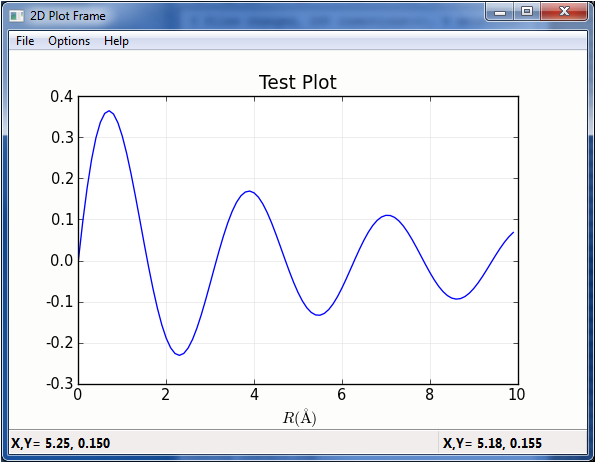
\includegraphics{basic_screenshot.png}

The configuration window (Options-\textgreater{}Configuration or Ctrl-K) for this plot looks
like this:

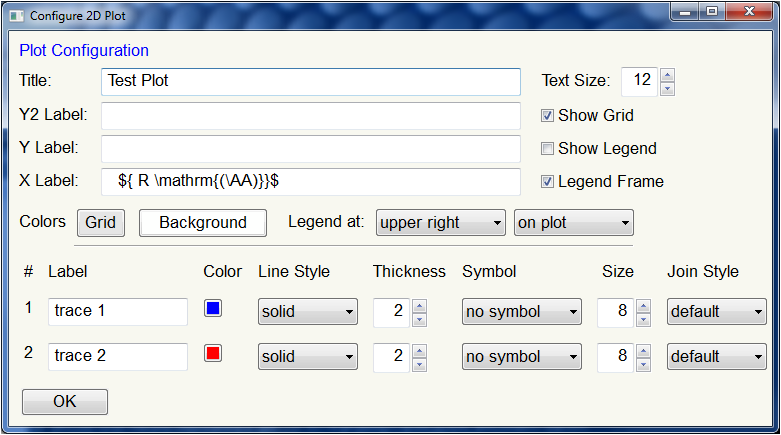
\includegraphics{configuration_frame.png}

where all the options there will dynamically change the plot in the PlotPanel.


\chapter{\texttt{ImagePanel}:  A wx.Panel for Image Display}
\label{imagepanel:imagepanel-a-wx-panel-for-image-display}\label{imagepanel::doc}


\renewcommand{\indexname}{Index}
\printindex
\end{document}
